% !TEX root =  ../master.tex
\chapter{Anforderungsanalyse} % TODO: Das hier ist noch etwas durcheinander
\section{Abgrenzung}
\subsection{Abgrenzung des Funktionsumfangs}\label{sub:abgrenzung}
Im Bereich Bildung gibt es viele Möglichkeiten, wie Hochschulen und Studenten unterstützt werdem können.
Primär gibt es hierbei 4 Ebenen, auf denen Aktionen stattfinden können:
\begin{center}
	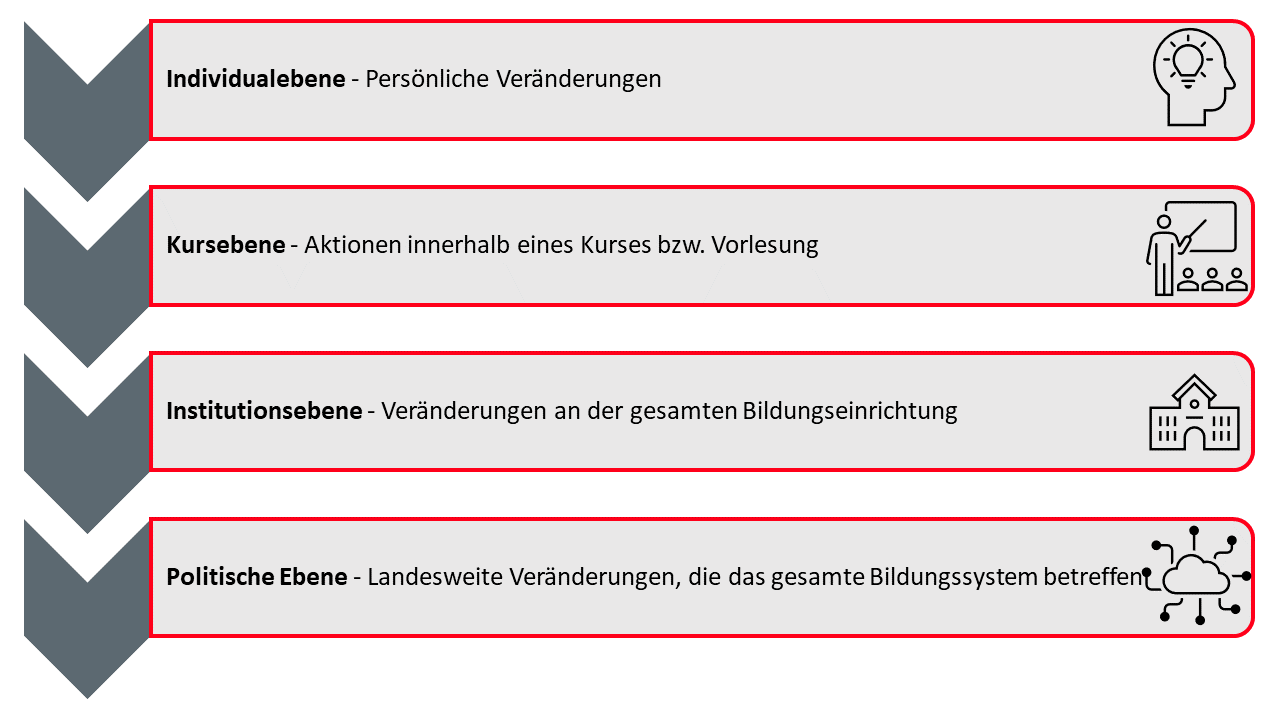
\includegraphics[width=\linewidth, keepaspectratio]{img/4LA.png}
\end{center}
Dieser Graphik kann entnommen werden, dass die Ebenen unterschiedliche Anforderungen mit sich bringen. Um auf politischer Ebene Daten miteinander zu verbinden braucht es entweder in den darunterliegenden Ebenen einheitliche Systeme oder ein weiteres System, das die unterschiedlichen Daten zusammenführt. Die Umsetzung solcher Lösungen bringt in der Regel viel Abstimmungs- und Überzeugungsaufwand mit sich, sodass diese sehr zeitintensiv ist. Da die Anwendung aber möglichst schnell krisenbeeinträchtigte Studenten unterstützten sollte, musste diese Ebene bei der Entwicklung zunächst vernachlässigt werden.

Die Institutionsebene beschreibt das Management von Ressourcen innerhalb der Hochschule. Besonders der Austausch und die Weiterbildung zwischen Dozenten ist hierbei ein wichtiger Aspekt. Problematisch ist aber die Identifizierung von Anforderungen aller Studienrichtungen. So besitzen technische Studiengänge andere Bedürfnisse als wirtschaftlich orientierte Studiengänge. Außerdem haben die einzelnen Fakultäten bereits unterschiedliche Erfahrungen mit dem Thema Learning Analytics gemacht und dementsprechend unterschiedliche Standpunkte und Fortschritte zu verzeichnen. Aus diesem Grund konnte auch diese Ebene nicht genauer beachtet werden.

Stattdessen wird sich in dieser Arbeit auf die Entwicklung einer Anwendung mit dem Schwerpunkt auf der Kurs- und der Individualebene fokussiert.
Die Kursebene dient zur Weitergabe von Lernmaterialien, die eine Vorlesung ergänzen. Außerdem bündelt sie für einen Kurs geltende Informationen, die ansonsten jeder Studierende einzeln für sich einarbeiten und berücksichtigen müsste. Dies soll einen direkten Einfluss auf die Individualebene haben und den individuellen Studenten fördern. Ziel ist es, den Studenten beim Lernen zu unterstützen, administrative Aufwände zu reduzieren und das Verständnis der in der Vorlesung vermittelten Informationen zu fördern.  

Durch diesen Fokus entfallen einige übergeordnete Auswertungsmöglichkeiten mit Methoden aus dem Bereich Data Mining, da für sie eine breitere Datengrundlage nötig wäre. Wir sind allerdings der Überzeugung, dass die Mgölichkeit der Auswertung von Lernfortschritten nicht der primäre Grund für die Entwicklung einer Anwendung sein sollte. Dies lässt sich vor allem damit begründen, dass die Quantität und Qualität der erhobenen Daten stark mit dem Mehrwert und dem damit verbunden Nutzerverhalten der Studenten zusammenhängt. Aus diesem Grund verfolgen wir das Ziel, eine auf die Anforderungen der Stundenten angepasste Anwendung zu liefern, die für die Studenten einen wirklichen Mehrwert darstellt und daher freiwillig und gerne von ihnen genutzt wird. Dadurch fallen implizit mehr Lerndaten an, die dann anonym ausgewertet werden können und eine höhere Repräsentativität ermöglichen. Sollte sich die Anwendung für Nutzer als vorteilhaft erweisen, kann die Anwendung aufgrund ihres technischen Designs ohne Probleme um Funktionalitäten aus anderen Ebenen erweitert werden und somit kontinuierlich wachsen.



% TODO: Können Wir vielleicht noch einen User Acceptance Test machen?

% TODO: Also bauen wir einen Export? Das wäre gut, dann können wir das schreiben. Aber da müssen wir mal schauen. Vordefinierte Auswertungen, Berechnungen wird es allerdings aufgrund der gewählten Abgrenzungen erst einmal nicht geben.
Die von Beginn an zu Verfügung stehenden Daten sollen im Ersten Schritt in einem auswertungstauglichen Format zur Verfügung gestellt werden. Die genauen Details werden später im Abschnitt Konzeption betrachtet. Wichtig ist uns hierbei jedoch, dass die Anonymität der einzelnen Nutzer geschützt bleibt und keine personenbezogenen Daten weitergegeben werden. Außerdem soll der Export dieser Daten nur den Dozenten eines Kurses vorbehalten sein. Aufgrund der vorgenommenen Themenabgrenzung muss jedoch die Auswertung selbst, inklusive der Auswahl der Daten und Methoden, vorerst noch durch die Dozierenden vorgenommen werden. 

% TODO: Abgrenzung zu anderen Werkzeugen
\subsection{Abgrenzung zu anderen Anwendungen}
Im Hochschulkontext kommen bereits mehrere Systeme zum Einsatz.
Die primäre Plattform bildet \enquote{Moodle}.
Moodle ist eine Lernplattform, in dem Nutzer Kurse, Kalender, Foren und ähnliche Funktionen erstellen können, die zur Steuerung und Verwaltung von Vorlesungen herangezogen werden können.
Trotz des recht umfangreichen Funktionsumfangs besitzt die Anwendung aber einige Nachteile.
So berichten viele Nutzer (Studenten, Dozenten und Unternehmensbetreuer) von sehr schlechter Bedienbarkeit und Unübersichtlichkeit.
Zusätzlich weißt die Datenschutzerklärung darauf hin, dass umfangreich Daten, z.\,B. \enquote{ob und wie sie [Nutzer] in Workshops mitgewirkt haben}, gesammelt werden können.\autocites{moodleTermsOfServiceDHBW}{moodleTermsOfService}
Aus Datenschutzrechtlichen Gründen werden aktuell die Learning Analytics Erweiterungen und andere Möglichkeiten der Kursmanagement- und Lernplattform Moodle nicht genutzt.

Ein weiteres Werkzeug, welches im Hochschulkontext verwendet wird, ist \enquote{Dualis}.
Diese Anwendung gibt aber nur Auskunft über Bewertungen.
Anwender können damit erstes Feedback zu ihren Klausuren erhalten, sobald sie Klausuren bereits beschrieben haben.
Somit besitzen die Studenen vor der Klausur oft kein Feedback zu der von ihnen geleisteten Arbeit.

Darüber hinaus existieren Anstrengungen, weitere Anwendungen umzusetzen, die aber nicht den Prototyp-Status verlassen haben.
Ein Beispiel hierfür ist die MyLA-Anwendung.\autocite{mylaGithub}
Für Dozenten gibt es die Möglichkeit, Umfragen zu erstellen und die Ergebnisse mit ihren Studierenden zu teilen. Diese haben dadurch die Chance, ihre Meinung zur Vorlesung mitzuteilen, Gelerntes zu verinnerlichen oder auch Anmerkungen zu gestellten Fragen zu geben. Die Plattform ermöglicht es dabei, Umfragen als Vorlage zu speichern, sodass diese in unterschiedlichen Kursen verwendet werden können. Die Ergebnisse der Umfragen sind graphisch darstellbar.

Zur Evaluierung von gehaltenen Vorlesungen kommt das System zur Automation von Befragungen und Prüfungen evasys zum Einsatz. \autocite{evasys} Hier wird jedoch nur Feedback zu bereits gehaltenen Vorlesungen stichprobenartig eingeholt. Kurzfristige Anpassungen des Inhaltes, Vorgehens oder anderen Aspekten einer Vorlesung an die Anforderungen und Wünsche der Studenten sind aufgrund des Abfragezeitpunktes nicht mehr möglich. Insgesamt lässt sich feststellen, dass viele unterschiedliche Systeme zum Lernen und Erheben von Meinungsbildern an der DHBW Mannheim genutzt werden. Augenscheinlich sind diese aber weder miteinander verknüpft noch in ein übergeordnetes System integriert. Zumindest können wir aus unserem Studienalltag von mehreren Beispielen berichten, wo die gleichen Daten mehrfach abgegeben werden mussten.

% TODO: Hier noch einen Satz, alle anderen Anwendungen sind Käse, und dass wir das alles super toll machen























\section{Personas}


% -------------------------------------------------------
% 1. Student
% 2. Dozent
% -------------------------------------------------------
% Keine Ahnung, irgendwelche Bilder halt :D
% https://unsplash.com/photos/ZVo7vtXilCs
\subsection{Beispiel Student}

\begin{minipage}[t]{0.5\textwidth}
	\vspace{-4cm}
	\renewcommand{\arraystretch}{1.5}
	\begin{tabular}{l l}
		Name: & Stephan Student \\
		Alter: & 21 \\
		Tätigkeit: & Student Wirtschaftsinformatik \\
		IT-Skills: & 4/5 \hspace{-1cm} \begin{barchart}{5.0}
			\baritemNL{}{4}
		\end{barchart} \\
	\end{tabular}
\end{minipage}
\hfill
\begin{minipage}[t]{0.4\textwidth}
	\flushright
	
\includegraphics[width=0.70\textwidth]{img/carlos-lindner-ZVo7vtXilCs-unsplash.jpg}
\end{minipage}

Stephan ist ein typisches Beispiel für einen Studenten an der DHBW.
Er ist viel aktiv und wohnt aufgrund des Standortes seines Dualen Partners nicht in der Metropolregion Rhein-Neckar. Aus diesem Grund pendelt er regelmäßig zu Präsenzveranstaltungen und Klausuren. Da er für die Anfahrt lange Zeit in öffentlichen Verkehrsmitteln verbringt, möchte er nicht auf ein bestimmtes Endgerät angewiesen sein und sowohl von daheim am PC als auch in der vollen Straßenbahn am Handy lernen können.  Demnach möchte er ortsunabhängig stets eine Übersicht über seine anstehenden Klausuren erhalten und sich unterwegs auch auf diese vorbereiten können. Dabei ist es ihm wichtig, dass seine persönlichen Daten nicht weitergegeben werden und nicht zur Klausurbewertung oder ähnlichen Bewertungen herangezogen werden können.

Das möchte ich gerne haben:
\begin{itemize}
	\item Übersicht über meine Klausuren
	\item Auch unterwegs lernen können
	\item Anonymität
\end{itemize}

\subsection{Beispiel Dozent}
% https://unsplash.com/photos/TXxiFuQLBKQ
\begin{minipage}[t]{0.5\textwidth}
	\vspace{-4cm}
	\renewcommand{\arraystretch}{1.5}
	\begin{tabular}{l l}
		Name: & Dagmar Dozent \\
		Alter: & 35 \\
		Tätigkeit: & Dozentin für Finanzbuchhaltung \\
		IT-Skills: & 2/5 \hspace{-1cm} \begin{barchart}{5.0}
			\baritemNL{}{2}
		\end{barchart} \\
	\end{tabular}
\end{minipage}
\hfill
\begin{minipage}[t]{0.4\textwidth}
	\flushright
	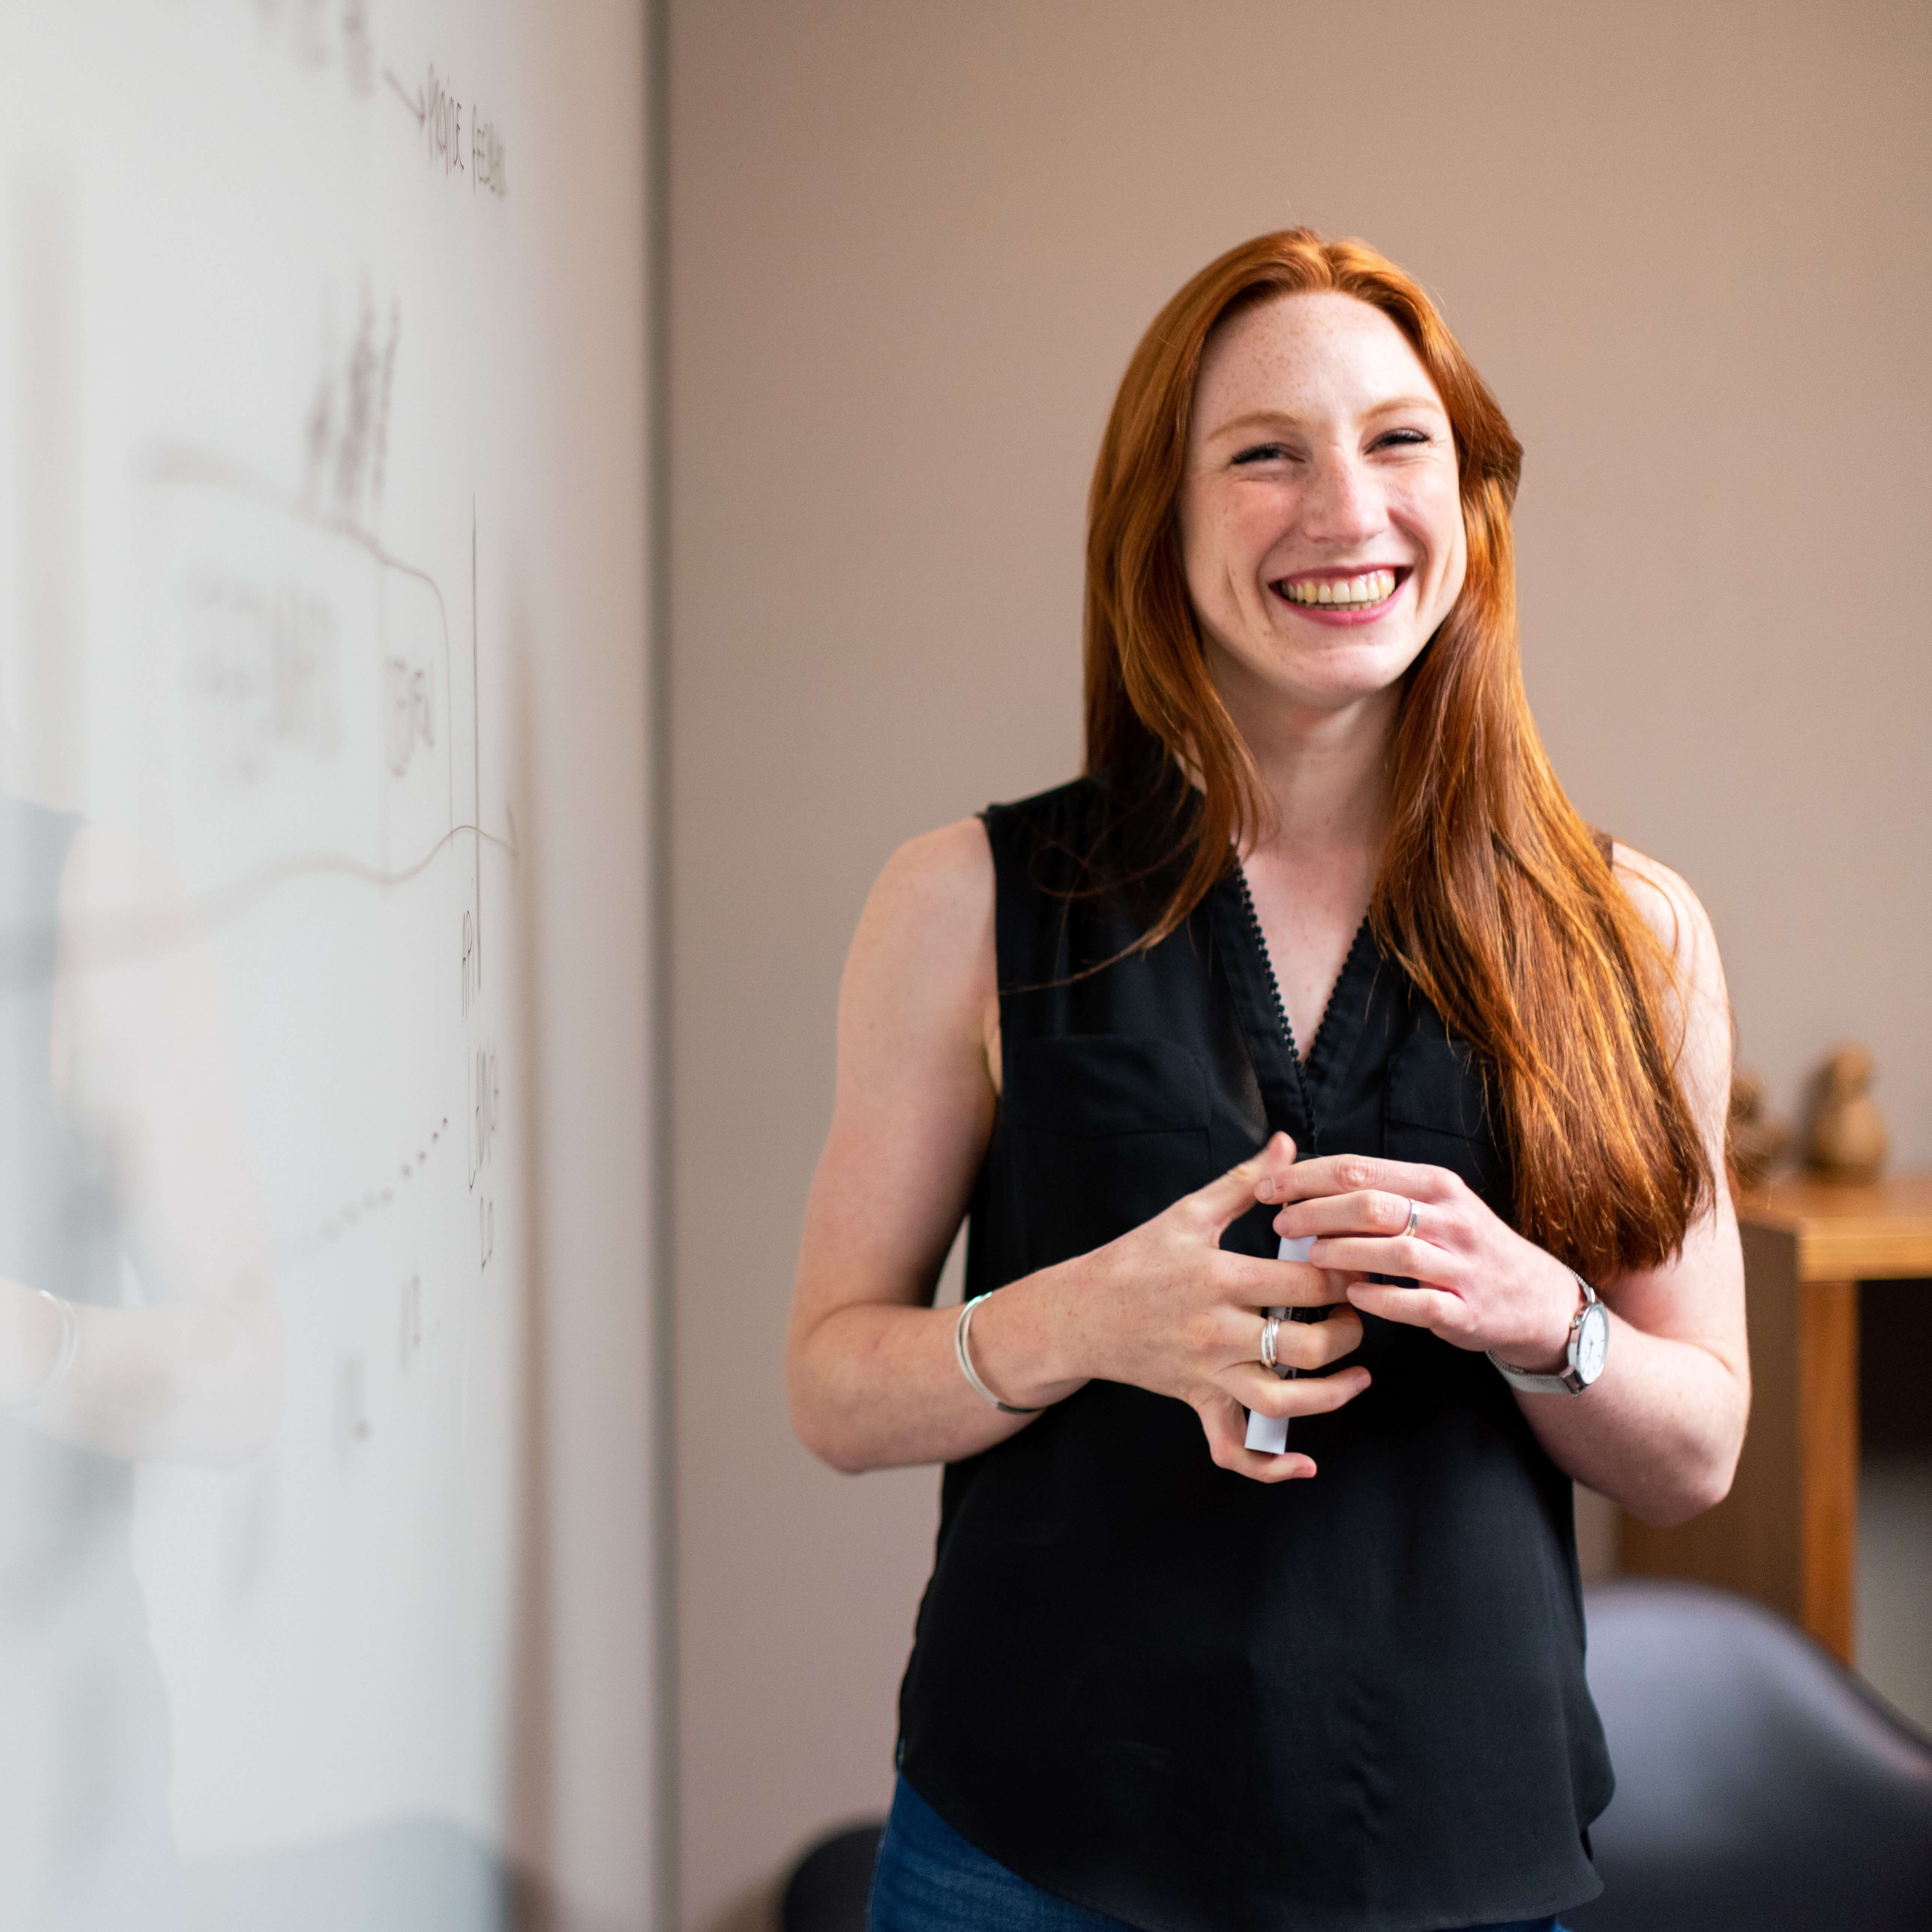
\includegraphics[width=0.70\textwidth]{img/thisisengineering-raeng-TXxiFuQLBKQ-unsplash.jpg}
\end{minipage}

Dagmar ist eine Dozentin für Wirtschaftsthemen, vorrangig Finanzbuchhaltung.
Als verantwortungsbewusste Person ist es ihr wichtig, dass Studenten auch außerhalb ihrer Vorlesung Unterstützung erhalten.
Aus diesem Grund möchte sie gerne weiterführende Informationen an ihre Studenten geben.
Gleichzeitig möchte sie gerne Feedback zu ihrer Vorlesung erhalten, um das Lernmaterial bestmöglich anpassen zu können.
Da sich allerdings ihre Kernkompetenzen außerhalb der IT befinden ist es ihr wichtig, dass sie die Anwendung unkompliziert und ohne lange Einführung nutzen kann. 


Das möchte ich gerne haben:
\begin{itemize}
	\item Informationen an alle Studenten des Kurses verteilen
	\item Feedback zum Kurs erhalten
	\item Intuitive Bedienung
\end{itemize}
% Generell Umfragen, .... alles erst reinschreiben, wenn wir das auch implementiert haben :)



















\section{Ist-Analyse}
Bevor die eigentliche Entwicklung starten kann, müssen die aktuellen Probleme und Verbesserungspotenziale analysiert werden.

Dozierende haben aktuell wenig Möglichkeiten zu erfahren, wie ihre Vorlesung in verschiedenen Kursen angenommen werden.
Besonders der Lernstand der Studierenden und die Stimmung innerhalb der Kurse sind nur schwer erfassbar.
Nach Aussage eines Dozenten wurde uns gesagt, dass dies besonders in Online-Vorlesungen problematisch ist.
Sofern man \enquote{nicht in fragende Gesichter schaut}, ist es oft schwer zu wissen, wann eine Fragestellung zu kompliziert ist.
Besonders die gegebene \enquote{Anonymität} der an der DHBW gehaltenen Online-Vorlesungen, bei denen im Regelfall kein Video der Teilnehmenden gestreamed wird, verschlechtert die Situation nochmals.
Dadurch kann eine Differenz zwischen dem gefühlten und dem tatsächlichen Leistungsstand entstehen, die sich dann erst in Klausuren negativ zeigen kann.
Aktuell (Dezember '20) finden das zweite Semester in Folge die Vorlesungen ausschließlich online statt. Wegen  der langen Dauer dieser Phase könnte eine Feedbackmöglichkeit für Dozierende nochmals relevanter sein.




\section{Anforderungsformulierung}

\subsection{Funktionale Anforderungen} 
Bei der Anforderungsanalyse gehen wir nach dem Motto "Von Studenten für Studenten" vor. Wir als Studenten der DHBW können sehr gut einschätzen, was uns das Studium erleichtern würde und wie wir uns in Bezug auf Klausuren und Prüfungen besser organisieren könnten. Mit einer Prozessierung und Automatisierung könnten Synergien genutzt werden, und auch andere Kommilitonen könnten von den für diese Veranstaltungen eingebrachten Anstrengungen profitieren.

Ziel dieser Arbeit ist es eine App zu entwickeln, die unabhängig von der Plattform als Web-Applikation oder im Browser genutzt werden kann.
Dabei sollen sowohl Studenten als auch Dozenten einen Zugang bekommen.
Wir setzen auf eine freiwillige Teilnahme. Die Anwendung soll durch ihre Funktionen und die intuitive Bedienbarkeit überzeugen und nicht durch einen Nutzungszwang.

Wir konnten die folgenden funktionalen Anforderungen definieren:
\begin{itemize}
    \item Anmeldung                         \\
        Es muss eine Möglichkeit geben, wie neue Studenten und Dozenten die Anwendung nutzen können.
        In der DHBW kommen mit jedem Semester neue Studenten und neue Dozenten.
        Aus diesem Grund muss es eine Möglichkeit geben, neue Nutzer für die Nutzung der Anwendung zu authorisieren.
        Eine Anmeldung kapselt außerdem die Daten einzelner Nutzer.
    \item Kurszuweisung                     \\
        In \autoref{sub:abgrenzung} wurde bereits beschrieben, dass die Kursebene abgedeckt wird.
        Aus diesem Grund muss es eine Möglichkeit geben, Studenten zu Kursen zuzuweisen.
        Kurse sollen dabei eine logische Abgrenzung bilden, sodass Studenten nicht den Lernstoff  verschiedener Vorlesungen durcheinander bringen.
    \item TODOs                             \\
        Bisher ist es schwer, einen Überblick über alle Aufgaben zu haben, die von Studenten zu erledigen sind.
        Besonders die Vielzahl an Vorlesungen, die sich in ihrem Aufbau und in der Prüfungsweise unterscheiden, erfordern unterschiedliche Vorbereitungen und damit TODOs.
        TODOs können dabei optional ein Fälligkeitsdatum besitzen, welches zur besseren Organisation der eingetragenen TODOs graphisch anzeigbar ist.
        So entsteht ein Kalender, mit dessen Hilfe  Kapazitätsengpässe rechtzeitig erkannt und durch Umplanen verhindert werden können.
	% TODO: Hier ist ein Teil reingerutscht der eigentlich mehr Theorei als ANforderung ist!
    \item Karteikarten                      \\
        Für eine bessere Prüfungsvorbereitungen können Karteikarten angelegt werden. Unterschiedliche wissenschaftliche Untersuchungen zeigen die Vorteile dieser Methode. Die Karteikarten sollen direkt in der App gelernt werden, sodass kein zusätzlicher Aufwand für das Abschreiben der Karten notwendig ist.

    \item Prüfungsterminübersicht           \\
        In der Anwendung soll es eine Übersicht aller Klausuren und anderen Prüfungsleistungen geben.
        Momentan wird dies über einen Google Kalender gehandhabt, welcher über eine Zwischeninstanz verwaltet wird.
        Da dieser Kalender direkt in der Anwendung angegeben ist, können zusätzliche Informationen (z.\,B. zugelassene Hilfsmittel) leichter kommuniziert werden und die zeitliche Differenz wird aufgehoben.

    \item Kursübergreifende Informationen   \\
        Besitzt ein Nutzer einen Account, soll er Kurse anlegen können, zu denen er Informationen wie  Prüfungstermine erfassen kann.
        Um zu verhindern, dass dieser organisatorische Aufwand von jedem Studenten einzeln durchgeführt werden muß, soll es zusätzlich eine Funktion geben, mit der Dozenten einen Kurs anlegen können.
        Den Kursen können initial bereits Prüfungstermine und Karteikarten mitgegeben werden.
        Somit entfällt die vielfache initiale Erstellung.
        Das Erstellen eines Kurses hat für den Dozenten den Vorteil, dass für diesen Kurs Daten zur Verfügung gestellt bekommt, die er zur Anpassung oder Evaluation seiner Vorlesung nutzen kann.
        Beispiele hierfür können sein Lerntypen der Studenten, Fortschritt beim Lernen der Karteikarten, etc.
    \item Rollendifferenzierung             \\
        Aus den bereits beschriebenen Anforderungen geht hervor, dass es eine Weise geben muss, wie Dozenten von Studenten unterschieden wird.
        Es soll verhindert werden, dass Studenten falsche Informationen bereitstellen können und so andere Studenten des gleichen Kurses schädigen.
        Aus diesem Grund sollen nur Dozenten Informationen bereitstellen können, die von mehreren Studenten eingesehen werden können.
    \item Übersichtliches Dashboard			\\
   		Die Anwendung soll erleichtern, den Überblick über die in nächster Zeit anstehenden Aufgaben und Tätigkeiten zu behalten. Dies ermöglichen die anstehenden Klausuren, eingetragene ToDos und Karteikarten, die am selben Tag zum Lernen empfohlen werden.
  
\end{itemize}

% Das ist das was ich grad realistisch sehe. Wenn wir noch mehr implementiert haben, dann können wir das gerne noch erweitern


\subsection{Nicht-Funktionale Anforderungen}
Neben den funktionalen Anforderungen gibt es auch einige nicht-funktionale Anforderungen, die beachtet werden müssen.
\begin{itemize}
    \item Barrierefreiheit		\\
        Um allen Nutzern unabhängig von ihren Einschränkungen oder technischen Möglichkeiten die uneingeschränkte Nutzung der Anwendung zu ermöglichen, sind für diese Anwendung einige Überlegungen angestellt worden. So soll sich die Sprache der Anwendung an den Spracheinstellungen des Webbrowsers auf dem Gerät des jeweiligen Nutzers orientieren. Darüber hinaus soll diese auch in der Anwendung selbst umgestellt werden können. Hierbei sollen alle Nutzergruppen angesprochen werden. Als potenzielle Nutzer seien hier Austausch-Studenten oder diejeingen Kommilitonen, die lieber in einer anderen Sprache arbeiten möchten, weil sie damit zum Beispiel die Inhalte leichter verstehen können, erwähnt. Das Standard-Design orientiert sich am Corporate Design der Dualen Hochschule Württemberg. Es soll jedoch einfach über ein Drop-Down Menü angepasst werden können, so dass auch Versionen mit erhöhtem Kontrast etc. erzeugt werden können bzw. das Layout nach den eigenen Präferenzen und Bedürfnissen gestaltet werden kann.
    \item Geschwindigkeit\\
        Für Nutzer ist die Geschwindigkeit besonders wichtig.
        Lang ladende Anwendungen sind nicht nur nervig in der Benutzung, sondern könnten sich in der hier entwickelten Anwendung negativ auf den Lernfortschritt auswirken. Lange Ladezeiten lenken beispielsweise ab und demotivieren die Nutzung der Anwendung.
        Über lange Ladezeiten beschweren sich in einer Umfrage mehr als 70\%, wobei 25\% aller Nutzer bereits bei 4 Sekunden die Seite verlassen.\autocite{loadingTimes}
        Aus diesem Grund sollte die Ladezeit gering gehalten werden.
    \item Persistenter Speicher             \\
        Informationen über Kurse müssen dauerhaft gespeichert und jederzeit abrufbar sein.
        Besonders kurz vor und nach einer Vorlesung wird die Nutzung der Anwendung voraussichtlich deutlich ansteigen.
        Auch bei Spitzenlast müssen alle Informationen stets zügig abrufbar sein.
    \item Responsives Design\\
        Die Anwendung sollte auf jeden Gerät vollständig funktional sein.
        Studenten nutzen häufig viele Geräte mit verschiedenen Bildschirmformaten.
        Besonders unterwegs oder in öffentlichen Verkehrsmitteln sind Mobilgeräte die primäre Wahl.
        Aus diesem Grund muss sich die Anwendung dynamisch an solche Geräte anpassen.
    \item Corporate Design\\
        Die DHBW besitzt ein einheitliches Design, an der man alle DHBWs und DHBW-Anwendungen erkennt \autocite{CD-DHBW}.
        Damit die Anwendung sich an die DHBW angliedert, sollte die Anwendung nahe an diesem Design sein.
        Besonders das Farbschema sollte dabei einheitlich sein. % TODO: Muss das wirklich sein, das sieht halt echt nicht gut aus. Ich mag das cosmic theme ganz gern
    \item Datenschutz\\
        Der Schutz von personenbezogenen Daten steht hier besonders im Vordergrund.
        Wie oben bereits festgestellt wurde, besitzen Anwendungen gegenwärtig problematische Datenschutzlagen.
        Aus diesem Grund soll die entwickelte Anwendung einen hohen Wert auf den Datenschutz legen und die Verarbeitung personenbezogener Daten auf ein Minimum reduzieren.
\end{itemize}



\subsection{Zusammenfassung}
Die gerade beschriebenen funktionalen und nicht-funktionalen Anforderungen sind noch übersichtlich und für die spätere Referenz in \autoref{tab:anforderungen} dargestellt.


\begin{table}[h]
    \centering
    \begin{tabularx}{.8\textwidth}{l|X}
        Nr.     & Beschreibung                              \\\hline
        F1      & Neue Nutzer können sich für die Nutzung anmelden                    \\
        F2      & Studenten können für Kurse eingeschrieben werden  \\
        F3      & Es können TODOs erstellt werden   \\
        F4      & Es kann mit Karteikarten gelernt werden  \\
        F5      & Prüfungstermine können eingetragen werden  \\
        F6      & Informationen können allen Studenten mitgeteilt werden  \\
        F7      & Es gibt eine Unterscheidung zwischen Studenten und Dozenten  \\
        F8      & Anstehenden Aufgaben und Prüfungen sollen übersichtlich dargestellt werden  \\\hline
        NF1     & Die Anwendung soll möglichst barrierefrei gestaltet werden\\
        NF2     & Anwendung lädt schnell                    \\
        NF3     & Daten jederzeit einsehbar                 \\
        NF4     & Anwendung funktioniert auf allen Geräten  \\
        NF5     & Anwendung ist am DHBW Design orientiert   \\
        NF6     & Personenbezogene Daten werden geschützt  \\
    \end{tabularx}
    \caption{Zusammengefasste Anforderungen}
    \label{tab:anforderungen}
\end{table}



